\documentclass{../vespers-booklet}
\usepackage{multicol}
\grechangestyle{abovelinestext}{\color{red}\itshape}

\begin{document}

\chapter*{First Vespers of the Sacred Heart of Jesus}

\begin{figure}[h!]
	\centering
	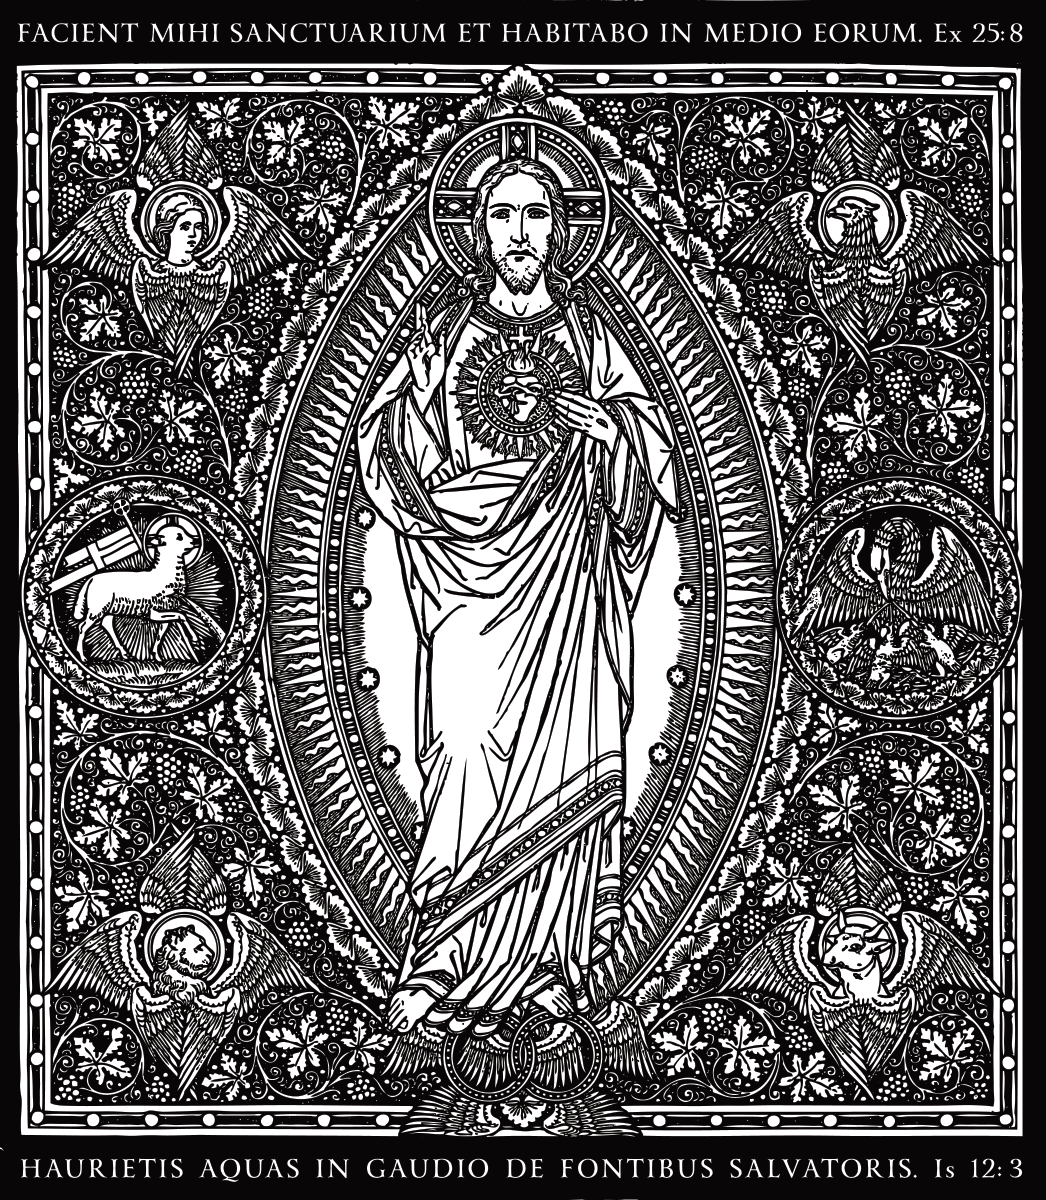
\includegraphics[width=0.8\textwidth]{Sacred_Heart_Line_Art}
\end{figure}

\pagebreak

\section*{Beginning of the Office}

\begin{rubricbox}

{\color{red}After the Celebrant arrives to the Predella, he kneels and silently prays the following:}

\end{rubricbox}

\begin{latinenglishsection}

\latinenglish{
	Aperi, Dómine, os meum ad benedicéndum nomen sanctum tuum: munda quoque cor meum ab ómnibus vanis, pervérsis et aliénis cogitatiónibus; intelléctum illúmina, afféctum inflámma, ut digne, atténte ac devóte hoc Offícium recitáre váleam, et exaudíri mérear ante conspéctum divínæ Majestátis tuæ. Per Christum Dóminum nostrum. Amen. 
	
	Dómine, in unióne illíus divínæ intentiónis, qua ipse in terris laudes Deo persolvísti, hanc tibi Horam persólvo.
}{
	Open, O Lord, my mouth to bless thy holy Name; cleanse also my heart from all vain, evil, and wandering thoughts; enlighten my understanding and kindle my affections; that I may worthily, attentively, and devoutly recite this Hour, and so be meet to be heard before the presence of thy divine Majesty. Through Christ our Lord. Amen.
	
	O Lord, in union with that divine intention wherewith thou, whilst here on earth, didst render praises unto God, I desire to offer this my Office of prayer unto thee.
}

\end{latinenglishsection}

\begin{rubricbox}

{\color{red}When the Celebrant stands, all \textbf{stand} and the Celebrant then is led to his sedilia (chair). After briefly sitting, he rises and says silently one \textit{Pater noster} (Our Father) and \textit{Ave Maria} (Hail Mary).
Then all make the Sign of the Cross with the Celebrant as he intones:}

\end{rubricbox}

\gresetinitiallines{1}
\gregorioscore{../common/deus-in-adjutorium-solemn}

\textit{
O God, come to my assistance.
{\color{red}\Rbar.}~O Lord, make haste to help me.
Glory be to the Father, and to the Son, and to the Holy Spirit,
as it was in the beginning, is now, and ever shall be, world without end. Amen.
Alleluia.}

\section*{Psalm 109}

\textit{\textnormal{Ant. 1.}  Put thy easy yoke upon all mankind, O Lord, and be thou ruler, even in the midst of thine enemies.
 \textnormal{Ps.} The Lord said to my Lord: Sit thou at my right hand.}
 
 \begin{rubricbox}

{\color{red}All remain standing throughout the first antiphon.
After the psalm is intoned by the Cantor, the Celebrant dons his biretta and all \textbf{sit} at the asterisk.}

\end{rubricbox}

\gresetinitiallines{1}
\gregorioscore{2025/ps109-antiphon}

\gresetinitiallines{0}
\gregorioscore{2025/ps109-intonation}

 \begin{latinenglishsection}

\latinenglish{

	2. Donec ponam ini\textbf{mí}cos \textbf{tu}os,~*
	scabéllum pe\textit{dum} \textit{tu}\textbf{ó}rum.

3. Virgam virtútis tuæ emíttet Dómi\textbf{nus} ex \textbf{Si}on:~*
	domináre in médio inimicó\textit{rum} \textit{tu}\textbf{ó}rum.

4. Tecum princípium in die virtútis tuæ in splendóri\textbf{bus} sanc\textbf{tó}rum:~*
	ex útero ante lucíferum \textit{gé}\textit{nu}\textbf{i} te.

5. Jurávit Dóminus, et non p{\oe}ni\textbf{té}\-bit \textbf{e}um:~*
	Tu es sacérdos in ætérnum secúndum órdi\textit{nem} \textit{Mel}\textbf{chí}se\-dech.

6. Dóminus a \textbf{dex}tris \textbf{tu}is,~*
	confrégit in die iræ \textit{su}\textit{æ} \textbf{re}ges.

7. Judicábit in natiónibus, im\textbf{plé}bit ru\textbf{í}nas:~*
	conquassábit cápita in ter\textit{ra} \textit{mul}\textbf{tó}rum.

8. De torrénte in \textbf{vi}a \textbf{bi}bet:~*
	proptérea exal\textit{tá}\textit{bit} \textbf{ca}put.

9. \textit{(bow)} Glória \textbf{Pa}tri, et \textbf{Fí}lio,~*
	et Spirí\textit{tu}\textit{i} \textbf{Sanc}to.

10. \textit{(rise)} Sicut erat in princípio, et \textbf{nunc}, et \textbf{sem}per,~*
	et in s\'{\ae}cula sæcu\textit{ló}\textit{rum}. \textbf{A}men.

}{
	% 1. The Lord said to my Lord: Sit thou at my right hand:

2. Until I make thy enemies thy footstool.
 
3. The Lord will send forth the sceptre of thy power out of Sion: rule thou in the midst of thy enemies.
 
4. With thee is the principality in the day of thy strength: in the brightness of the saints:
 from the womb before the day star I begot thee.
 
5. The Lord hath sworn, and he will not repent: Thou art a priest for ever according to the order of Melchisedech.
 
6. The Lord at thy right hand hath broken kings in the day of his wrath.

7. He shall judge among nations, he shall fill ruins: he shall crush the heads in the land of the many.

8. He shall drink of the torrent in the way: therefore shall he lift up the head. 

Glory be.
}

\end{latinenglishsection}

%\begin{rubricbox}
%
%{\color{red}The antiphon is repeated: \textit{Suávi iugo tuo\dots}}
%
%\end{rubricbox}

\gresetinitiallines{1}
\gregorioscore{2025/ps109-antiphon_nc}

\begin{rubricbox}

{\color{red} The remaining Psalms are all said in the same manner as the first, except that all remain seated (except the Cantor who intones the given Antiphon and Psalm verse; for both, the Cantor rises to intone and sits at the asterisk).}

\end{rubricbox}

\section*{Psalm 110}

\textit{\textnormal{Ant. 2.} This merciful and gracious Lord hath given Meat unto them that fear him.
 \textnormal{Ps.} I will praise thee, O Lord, with my whole heart; in the council of the just: and in the congregation.}

\gresetinitiallines{1}
\gregorioscore{2025/ps110-antiphon}

\gresetinitiallines{0}
\gregorioscore{2025/ps110-intonation}

 \begin{latinenglishsection}

\latinenglish{
	
	2. Magna ópera \textbf{Dó}mini:~* exquisíta in omnes voluntá\textit{tes} \textbf{e}jus.

3. Conféssio et magnificéntia opus \textbf{e}jus:~* et justítia ejus manet in s\'{\ae}cu\textit{lum} \textbf{s\'{\ae}}culi.

4. Memóriam fecit mirabílium suórum,~\GreDagger\ miséricors et miserátor \textbf{Dó}minus:~* escam dedit timén\textit{ti}\textbf{bus} se.

5. Memor erit in s\'{\ae}culum testaménti \textbf{su}i:~* virtútem óperum suórum annuntiábit pópu\textit{lo} \textbf{su}o:

6. Ut det illis hereditátem \textbf{gén}ti\-um:~* ópera mánuum ejus véritas, et \textit{ju}\textbf{dí}cium.

7. Fidélia ómnia mandáta ejus:~\GreDagger\ confirmáta in s\'{\ae}culum \textbf{s\'{\ae}}culi,~* facta in veritáte et æ\textit{qui}\textbf{tá}te.

8. Redemptiónem misit pópulo \textbf{su}o:~* mandávit in ætérnum testamén\textit{tum} \textbf{su}um.

9. Sanctum, et terríbile nomen \textbf{e}jus:~* inítium sapiéntiæ ti\textit{mor} \textbf{Dó}\-mini.

10. Intelléctus bonus ómnibus faciéntibus \textbf{e}um:~* laudátio ejus manet in s\'{\ae}cu\textit{lum} \textbf{s\'{\ae}}culi.

\textit{(bow)} Glória Patri, et \textbf{Fí}lio,~* et Spirítu\textit{i} \textbf{Sanc}to.

\textit{(rise)} Sicut erat in princípio, et nunc, et \textbf{sem}per,~* et in s\'{\ae}cula sæculó\textit{rum}. \textbf{A}men.

}{
 	 1. I will praise thee, O Lord, with my whole heart; in the council of the just: and in the congregation.
 
 2. Great are the works of the Lord: sought out according to all his wills.
 
 3. His work is praise and magnificence: and his justice continueth for ever and ever.
 
 4.  He hath made a remembrance of his wonderful works, being a merciful and gracious Lord: he hath given food to them that fear him. 	
 
 5. He will be mindful for ever of his covenant: he will shew forth to his people the power of his works.
 
 6. That he may give them the inheritance of the Gentiles: the works of his hands are truth and judgment.
 
 7. All his commandments are faithful: confirmed for ever and ever, made in truth and equity.
 
 8. He hath sent redemption to his people: he hath commanded his covenant for ever.
 
 9. Holy and terrible is his name: the fear of the Lord is the beginning of wisdom.
 
 10. A good understanding to all that do it: his praise continueth for ever and ever. 
}

\end{latinenglishsection}

%\begin{rubricbox}
%
%{\color{red}The antiphon is repeated: \textit{Miséricors\dots}}
%
%\end{rubricbox}

\gresetinitiallines{1}
\gregorioscore{2025/ps110-antiphon_nc}

\section*{Psalm 111}

\textit{\textnormal{Ant. 3.} Unto the godly there ariseth up a light in the darkness even the Lord merciful and gracious.
 \textnormal{Ps.} Blessed is the man that feareth the Lord: * he shall delight exceedingly in his commandments.}

\gresetinitiallines{1}
\gregorioscore{2025/ps111-antiphon}

\gresetinitiallines{0}
\gregorioscore{2025/ps111-intonation}

 \begin{latinenglishsection}

\latinenglish{
	
	2. Potens in terra erit \textbf{se}men \textbf{e}jus:~*
	generátio rectórum be\textbf{ne}di\textbf{cé}tur.

3. Glória, et divítiæ in \textbf{do}mo \textbf{e}jus:~*
	et justítia ejus manet in \textbf{s\'{\ae}}culum \textbf{s\'{\ae}}culi.

4. Exórtum est in ténebris \textbf{lu}men \textbf{rec}tis:~*
	miséricors, et mise\textbf{rá}tor, et \textbf{jus}tus.

5. Jucúndus homo qui miserétur et cómmodat,~\GreDagger\
	dispónet sermónes suos \textbf{in} ju\textbf{dí}cio:~*
	quia in ætérnum non \textbf{com}mo\textbf{vé}bitur.

6. In memória ætérna \textbf{e}rit \textbf{jus}tus:~*
	ab auditióne mala \textbf{non} ti\textbf{mé}bit.

7. Parátum cor ejus speráre in Dómino,~\GreDagger\
	confirmátum \textbf{est} cor \textbf{e}jus:~*
	non commovébitur donec despíciat ini\textbf{mí}cos \textbf{su}os.

8. Dispérsit, dedit paupéribus:~\GreDagger\
	justítia ejus manet in \textbf{s\'{\ae}}culum \textbf{s\'{\ae}}\-culi,~*
	cornu ejus exaltábi\textbf{tur} in \textbf{gló}ria.

9. Peccátor vidébit, et irascétur,~\GreDagger\
	déntibus suis fremet \textbf{et} ta\textbf{bé}scet:~*
	desidérium pecca\textbf{tó}rum per\textbf{í}bit.

\textit{(bow)} Glória \textbf{Pa}tri, et \textbf{Fí}lio,~*
	et Spi\textbf{rí}tui \textbf{Sanc}to.

\textit{(rise)} Sicut erat in princípio, et \textbf{nunc}, et \textbf{sem}per,~*
	et in s\'{\ae}cula sæcu\textbf{ló}rum. \textbf{A}men.

}{
 	1. Blessed is the man that feareth the Lord: he shall delight exceedingly in his commandments.

2. His seed shall be mighty upon earth: the generation of the righteous shall be blessed.

3. Glory and wealth shall be in his house: and his justice remaineth for ever and ever.

4. To the righteous a light is risen up in darkness: he is merciful, and compassionate and just.

5. Acceptable is the man that sheweth mercy and lendeth: he shall order his words with judgment:
because he shall not be moved for ever.

6. The just shall be in everlasting remembrance: he shall not fear the evil hearing.

7. His heart is ready to hope in the Lord: his heart is strengthened, he shall not be moved until he look over his enemies.

8. He hath distributed, he hath given to the poor: his justice remaineth for ever and ever: his horn shall be exalted in glory.

9. The wicked shall see, and shall be angry, he shall gnash with his teeth and pine away: the desire of the wicked shall perish. 
}

\end{latinenglishsection}

%\begin{rubricbox}
%
%{\color{red}The antiphon is repeated: \textit{Exórtum est\dots}}
%
%\end{rubricbox}

\gresetinitiallines{1}
\gregorioscore{2025/ps111-antiphon_nc}

\section*{Psalm 115}

\textit{\textnormal{Ant. 4.} What reward shall I give unto the Lord for all the benefits that he hath done unto me?
 \textnormal{Ps.} I have believed, therefore have I spoken; * but I have been humbled exceedingly.}

\gresetinitiallines{1}
\gregorioscore{2025/ps115-antiphon}

\gresetinitiallines{0}
\gregorioscore{2025/ps115-intonation}

 \begin{latinenglishsection}

\latinenglish{
	
	2. Ego dixi in excéssu \textbf{me}o:~* Omnis \textit{ho}\textit{mo} \textbf{men}dax.

3. Quid retríbuam \textbf{Dó}mino,~* pro ómnibus, quæ retrí\textit{bu}\textit{it} \textbf{mi}hi?

4. Cálicem salutáris ac\textbf{cí}piam:~* et nomen Dómini \textit{in}\textit{vo}\textbf{cá}bo.

5. Vota mea Dómino reddam coram omni pópulo \textbf{e}jus:~* pretiósa in conspéctu Dómini mors sanc\textit{tó}\textit{rum} \textbf{e}jus:

6. O Dómine, quia ego servus \textbf{tu}us:~* ego servus tuus, et fílius an\textit{cíl}\textit{læ} \textbf{tu}æ.

7. Dirupísti víncula mea:~{\color{red}\GreDagger}\ tibi sacrificábo hóstiam \textbf{lau}dis,~* et nomen Dómini \textit{in}\textit{vo}\textbf{cá}bo.

8. Vota mea Dómino reddam in conspéctu omnis pópuli \textbf{e}jus:~* in átriis domus Dómini, in médio tu\textit{i}, \textit{Je}\textbf{rú}salem.

{\color{red}\textit{(bow)}} Glória Patri, et \textbf{Fí}lio,~* et Spirí\textit{tu}\textit{i} \textbf{Sanc}to.

{\color{red}\textit{(rise)}} Sicut erat in princípio, et nunc, et \textbf{sem}per,~* et in s\'{\ae}cula sæcu\textit{ló}\textit{rum}. \textbf{A}men.

}{
 	%1. I have believed, therefore have I spoken; * but I have been humbled exceedingly.

2. I said in my excess: * Every man is a liar.

3. What shall I render to the Lord, * for all the things that he hath rendered to me?

4. I will take the chalice of salvation; * and I will call upon the name of the Lord.

5.  I will pay my vows to the Lord before all his people: * precious in the sight of the Lord is the death of his saints.

6.  O Lord, for I am thy servant: * I am thy servant, and the son of thy handmaid.

7. Thou hast broken my bonds: * I will sacrifice to thee the sacrifice of praise, and I will call upon the name of the Lord.

8.  I will pay my vows to the Lord in the sight of all his people: * in the courts of the house of the Lord, in the midst of thee, O Jerusalem.

Glory be
}

\end{latinenglishsection}

%\begin{rubricbox}
%
%{\color{red}The antiphon is repeated: \textit{Quid retríbuam\dots}}
%
%\end{rubricbox}

\gresetinitiallines{1}
\gregorioscore{2025/ps115-antiphon_nc}

\section*{Psalm 129}

\textit{\textnormal{Ant. 5.} With the Lord, there is mercy, and with him is plenteous redemption.
 \textnormal{Ps.} Out of the depths I have cried to thee, O Lord: * Lord, hear my voice.}

\gresetinitiallines{1}
\gregorioscore{2025/ps129-antiphon}

\gresetinitiallines{0}
\gregorioscore{2025/ps129-intonation}

 \begin{latinenglishsection}

\latinenglish{
	
	2. Fiant aures tuæ \textit{in}\textit{ten}\textbf{dén}tes:~* in vocem depreca\textit{ti}\textit{ó}\textit{nis} \textbf{me}æ.

3. Si iniquitátes observá\textit{ve}\textit{ris}, \textbf{Dó}mine:~* Dómine, \textit{quis} \textit{sus}\textit{ti}\textbf{né}bit?

4. Quia apud te propiti\textit{á}\textit{ti}\textbf{o} est:~* et propter legem tuam sustí\textit{nu}\textit{i} \textit{te}, \textbf{Dó}mine.

5. Sustínuit ánima mea in \textit{ver}\textit{bo} \textbf{e}jus:~* sperávit ánima \textit{me}\textit{a} \textit{in} \textbf{Dó}mino.

6. A custódia matutína us\textit{que} \textit{ad} \textbf{noc}tem:~* speret Is\textit{ra}\textit{ël} \textit{in} \textbf{Dó}mino.

7. Quia apud Dóminum mi\textit{se}\textit{ri}\textbf{cór}dia:~* et copiósa apud \textit{e}\textit{um} \textit{red}\textbf{émp}tio.

8. Et ipse réd\textit{i}\textit{met} \textbf{Is}raël:~* ex ómnibus iniqui\textit{tá}\textit{ti}\textit{bus} \textbf{e}jus.

\textit{(bow)} Glória Pa\textit{tri}, \textit{et} \textbf{Fí}lio,~* et Spi\textit{rí}\textit{tu}\textit{i} \textbf{Sanc}to.

\textit{(rise)} Sicut erat in princípio, et \textit{nunc}, \textit{et} \textbf{sem}per,~* et in s\'{\ae}cula sæ\textit{cu}\textit{ló}\textit{rum}. \textbf{A}men.

}{
 	%1. Out of the depths I have cried to thee, O Lord: * Lord, hear my voice.

2. Let thy ears be attentive, to the voice of my supplication.

3. If thou, O Lord, wilt mark iniquities: Lord, who shall stand it.

4. For with thee there is merciful forgiveness: and by reason of thy law, I have waited for thee, O Lord.

5. My soul hath relied on his word: my soul hath hoped in the Lord.

6. From the morning watch even until night, let Israel hope in the Lord.

7. Because with the Lord there is mercy: and with him plentiful redemption.

8. And he shall redeem Israel * from all his iniquities.

Glory be.

}

\end{latinenglishsection}

%\begin{rubricbox}
%
%{\color{red}The antiphon is repeated: \textit{Apud Dóminum\dots}}
%
%\end{rubricbox}

\gresetinitiallines{1}
\gregorioscore{2025/ps129-antiphon_nc}

\vfill\pagebreak

\section*{Little Chapter (Ephesians 3:8-9)}

\textit{\color{red}The Celebrant hands his biretta to the MC. \textbf{All stand.} The Celebrant leads the Little Chapter:}

\begin{latinenglishsection}

\latinenglish{
	Fratres: Mihi ómnium sanctórum mínimo data est grátia hæc, {\color{red}\GreDagger}\ in géntibus evangelizáre investigábiles divítias Christi; {\color{red}*}\ et illumináre omnes, quæ sit dispensátio sacraménti abscónditi a s\'{\ae}culis in Deo.\\
	{\color{red}\Rbar.}~Deo grátias.
}{
	Brethren: Unto me, who am less than the least of all saints, is this grace given, that I should preach among the Gentiles the unsearchable riches of Christ; and to make all men see what is the fellowship of the Mystery, which from the beginning of the world hath been hid in God.\\
	{\color{red}\Rbar.}~Thanks be to God.
}

\end{latinenglishsection}

\section*{Hymn}

\textit{\color{red}\textbf{All remain standing.} A Cantor quietly pre-intones the Hymn for the Celebrant. The Celebrant then intones the Hymn up to the asterisk. Afterwards, each verse of the Hymn is sung by a different side, until all join together for the final verse:}

\gresetinitiallines{1}
\gregorioscore{2025/hymn_en_ut_superba}

{\itshape
	1. Lo, how the savage crew
	Of our proud sins hath rent
	The heart of our all-gracious God,
	That heart so innocent.

	2. The soldier's quivering lance
	Our guilt it was that drave,
	Our wicked deeds that to its point
	Such cruel sharpness gave.
	
	3. O wounded heart, whence sprang
	The Church, the Saviour's bride;
	Thou door of our salvation's ark
	Set in its mystic side.
	
	4. Thou holy fount, whence flows
	The sacred sevenfold flood,
	Where we our filthy robes may cleanse
	In the Lamb's saving blood:
	
	5. By sorrowful relapse,
	thee will we rend no more;
	But like the flames, those types of love,
	Strive heavenward to soar.
	
	6. Father and Son supreme
	And Spirit, hear our cry;
	Whose is the kingdom, praise and power,
	Through all eternity.
	Amen.
}

%\vfill\pagebreak

\textit{\color{red}The Cantor says the following:}
\gresetinitiallines{0}
\gabcsnippet{
(c3) <c><sp>V/</sp>.</c> Tól(h)li(h)te(h) ju(h)gum(h) me(h)um(h) su(hi)per(h) vos,(h'_) (,) et(h) dí(h')sci(f)te(e) a(fh_) me.(hiH'Ghih.ghG'FE'fggf.) (::)
}

\textit{\color{red}\textbf{All reply} as follows:}
\gresetinitiallines{0}
\gabcsnippet{
(c3) <c><sp>R/</sp>.</c> Qui(h)a(h) mi(hi)tis(h) sum(h'_) (,) et(h) hú(h')mi(f)lis(e) Cor(fh_)de.(hiH'Ghih.ghG'FE'fggf.) (::)
}

\textit{{\color{red}\Vbar.}~Take my yoke upon you, and learn of me.
{\color{red}\Rbar.}~For I am meek and lowly in Heart..}

\section*{Magnificat}

\textit{\textnormal{Ant Magn.}  I am come to send Fire on the earth, and what will I, but that it be kindled?
\textnormal{Cant.} My soul doth magnify the Lord: and my spirit hath rejoiced in God my Saviour.
}

\begin{rubricbox}

{\color{red}A Cantor again pre-intones the Magnificat antiphon for the Celebrant. The Celebrant then intones up to the asterisk, after which all \textbf{sit} and join in singing. The altar is incensed as at Mass.}

\end{rubricbox}

\gresetinitiallines{1}
\gregorioscore{2025/magnificat-antiphon}

\begin{rubricbox}

{\color{red}All \textbf{stand} and make the sign of the cross with the cantor.}

\end{rubricbox}

\gresetinitiallines{0}
\gregorioscore{2025/magnificat-intonation}

 \begin{latinenglishsection}

\latinenglish{	
	3. \textit{Quia} respéxit humilitátem an\textbf{cíl}læ \textbf{su}æ:~* ecce enim ex hoc beátam me dicent omnes gene\textit{ra}\textit{ti}\textbf{ó}nes.

4. \textit{Quia} fecit mihi \textbf{ma}gna qui \textbf{pot}ens est:~* et sanctum \textit{no}\textit{men} \textbf{e}jus.

5. \textit{Et mi}sericórdia ejus a progénie \textbf{in} pro\textbf{gé}nies~* timén\textit{ti}\textit{bus} \textbf{e}um.

6. \textit{Fecit} poténtiam in \textbf{brá}chio \textbf{su}o:~* dispérsit supérbos mente \textit{cor}\textit{dis} \textbf{su}i.

7. \textit{Depó}suit pot\textbf{én}tes de \textbf{se}de,~* et exal\textit{tá}\textit{vit} \textbf{hú}miles.

8. \textit{Esu}riéntes im\textbf{plé}vit \textbf{bo}nis:~* et dívites dimí\textit{sit} \textit{in}\textbf{á}nes.

9. \textit{Suscé}pit Israël \textbf{pú}erum \textbf{su}um,~* recordátus misericór\textit{di}\textit{æ} \textbf{su}æ.

10. \textit{Sicut} locútus est ad \textbf{pa}tres \textbf{nos}tros,~* Abraham et sémini e\textit{jus} \textit{in} \textbf{s\'{\ae}}cula.

11. {\color{red}\textit{(bow)}} \textit{Glóri}a \textbf{Pa}tri, et \textbf{Fí}lio,~* et Spirí\textit{tu}\textit{i} \textbf{Sanc}to.

12. {\color{red}\textit{(rise)}} \textit{Sicut} erat in princípio, et \textbf{nunc}, et \textbf{sem}per,~* et in s\'{\ae}cula sæcu\textit{ló}\textit{rum}. \textbf{A}men.


}{	
	1. My soul doth magnify the Lord.

2. And my spirit hath rejoiced in God my Saviour.

3. Because he hath regarded the humility of his handmaid; for behold from henceforth all generations shall call me blessed.

4. Because he that is mighty, hath done great things to me; and holy is his name.

5. And his mercy is from generation unto generations, to them that fear him.

6. He hath shewed might in his arm: he hath scattered the proud in the conceit of their heart.

7. He hath put down the mighty from their seat, and hath exalted the humble.

8. He hath filled the hungry with good things; and the rich he hath sent empty away.

9. He hath received Israel his servant, being mindful of his mercy: 

10. As he spoke to our fathers, to Abraham and to his seed for ever. 
}

\end{latinenglishsection}

\gresetinitiallines{1}
\gregorioscore{2025/magnificat-antiphon_e}

\section*{Collect}

\textit{\color{red}\textbf{All stand.} The Celebrant leads the collect:}

\begin{latinenglishsection}

\latinenglish{
	{\color{red}\Vbar.}~Dóminus vobíscum.\\
	{\color{red}\Rbar.}~Et cum spíritu tuo.
	
	Orémus.\\
	Deus, qui nobis in Corde Fílii tui, nostris vulneráto peccátis, infinítos dilectiónis thesáuros misericórditer largíri dignáris; concéde, qu\'{\ae}sumus, ut illi devótum pietátis nostræ præstántes obséquium, dignæ quoque satisfactiónis exhibeámus offícium.
	Per eúmdem Dóminum nostrum Jesum Christum Fílium tuum, qui tecum vivit et regnat in unitáte Spíritus Sancti, Deus, per ómnia s\'{\ae}cula sæculórum.
	
	{\color{red}\Rbar.}~Amen.
}{
	{\color{red}\Vbar.}~The Lord be with you.\\
	{\color{red}\Rbar.}~And with thy spirit.
	
	Let us pray.\\
	O God, who hast suffered the Heart of thy Son to be wounded by our sins, and in that very Heart hast bestowed on us the abundant riches of thy love: grant that the devout homage of our hearts, which we render unto him, may of thy mercy be deemed a recompence acceptable in thy sight.
	Through the same Jesus Christ, thy Son, Our Lord, Who liveth and reigneth with thee in the unity of the Holy Ghost, God, world without end.
	
	{\color{red}\Rbar.}~Amen.
}
\end{latinenglishsection}

%\textit{\color{red}For commemorations, the Cantor intones the antiphon and says the responsorial prayer afterwards. The Officiant prays the associated collect.}
%
%\pagebreak
%
%\section*{Commemoration of St. John and Paul, Martyrs (June 26)}
%
%\textit{\textnormal{Ant.} Theirs is the kingdom of heaven, who despising a worldy life have attained the rewards of the kingdom,
%and have washed their robes in the Blood of the Lamb.}
%
%\gresetinitiallines{1}
%\gregorioscore{../commemorations/many-martyrs-1v}
%
%\begin{latinenglishsection}
%
%\latinenglish{
%	{\color{red}\Vbar.}~Lætámini in Dómino, et exsultáte justi.\\
%	{\color{red}\Rbar.}~Et gloriámini omnes recti corde.
%	
%	Orémus.\\
%	Qu\'{\ae}sumus, omnípotens Deus: ut nos gemináta lætítia hodiérnæ festivitátis excípiat, quæ de beatórum Joánnis et Pauli glorificatióne procédit; quos éadem fides et pássio vere fecit esse germános.
%	% Per Dóminum nostrum Jesum Christum, Fílium tuum: qui tecum vivit et regnat in unitáte Spíritus Sancti, Deus, per ómnia s\'{\ae}cula sæculórum.
%}{
%	{\color{red}\Vbar.}~Be glad in the Lord and rejoice, ye just.\\
%	{\color{red}\Rbar.}~And exult, all ye upright of heart.
%	
%	Let us pray.\\
%	Almighty God, fill us, we beseech thee, with the twofold gladness which doth flow down upon this bright day from the glory of thy blessed servants John and Paul, whom one faith and one suffering made to be brothers indeed.
%	% Through Jesus Christ, thy Son our Lord, Who liveth and reigneth with thee, in the unity of the Holy Ghost, God, world without end.
%}
%
%\end{latinenglishsection}
%
%\section*{Commemoration of the Octave of Corpus Christi}
%
%\textit{\textnormal{Ant.} How holy this feast in which Christ is our food; his passion is recalled; grace fills our hearts; and we receive a pledge of the glory to come. Alleluia.}
%
%\gresetinitiallines{1}
%\gregorioscore{../commemorations/an--o_sacrum_convivium--solesmes_1961.1}
%
%\begin{latinenglishsection}
%\latinenglish{
%	{\color{red}\Vbar.}~Panem de caelo praestitísti eis, allelúia.\\
%	{\color{red}\Rbar.}~Omne delectaméntum in se habéntem, allelúia.
%	
%	Orémus.\\
%	Deus, qui nobis sub Sacraménto mirábili passiónis tuæ memóriam reliquísti: tríbue, qu\'{\ae}sumus, ita nos Córporis et Sánguinis tui sacra mystéria venerári; ut redemptiónis tuæ fructum in nobis júgiter sentiámus: 
%	Qui vivis et regnas, cum Deo Patre in unitáte Spíritus Sancti, Deus, per ómnia s\'{\ae}cula sæculórum.
%	
%	{\color{red}\Rbar.}~Amen.
%}{
%	{\color{red}\Vbar.}~The merciful Lord hath instituted a memorial of his wondrous deeds.\\
%	{\color{red}\Rbar.}~He hath given Meat unto them that fear him.
%	
%	Let us pray.\\
%	O God, Who in this wonderful sacrament has left us a memorial of Thy passion: grant us, we beseech Thee, so to venerate the sacred mysteries of Thy Body and Blood, that we may ever perceive within us the fruit of Thy redemption. 
%	Who lives and reigns with God the Father in the unity of the Holy Spirit, God, forever and ever.
%	
%	{\color{red}\Rbar.}~Amen.
%}
%\end{latinenglishsection}
%
%\vfill\pagebreak

\textit{\color{red}The Celebrant leads the Benedicamus and all reply with `Deo grátias':}

\gresetinitiallines{1}
\gregorioscore{../common/benedicamus-1v-solemn}

\textit{\color{red}The Officiant leads the following:}

\begin{latinenglishsection}

\latinenglish{
	{\color{red}\Vbar.} Fidélium ánimæ, per misericórdiam Dei, requiéscant in pace. \\
	{\color{red}\Rbar.} Amen.
}{
	{\color{red}\Vbar.}~May the souls of the faithful departed, through the mercy of God, rest in peace.\\
	{\color{red}\Rbar.}~Amen.
}

\end{latinenglishsection}

\end{document}